\documentclass[12pt]{article}
\usepackage{graphicx}
\usepackage{enumitem}
\usepackage{amsmath}
\usepackage{gvv-book}
\usepackage{gvv}

\title{\textbf{1.8.25}}
\author{\textbf{EE25BTECH11008 - Anirudh M Abhilash}}
\date{September 12, 2025}

\begin{document}

\maketitle

\section*{Question}

Find a relation between $x$ and $y$ such that the point $\vec{P}(x,y)$ is equidistant from the points $\vec{A}(7,1)$ and $\vec{B}(3,5)$.

\section*{Solution}

Let 
\[
\vec{P} = \myvec{x \\ y}, \quad \vec{A} = \myvec{7 \\ 1}, \quad \vec{B} = \myvec{3 \\ 5}.
\]

Since $\vec{P}$ is equidistant from $\vec{A}$ and $\vec{B}$,
\[
\|\vec{P} - \vec{A}\| = \|\vec{P} - \vec{B}\|.
\]

Squaring both sides and using the inner product,
\begin{align}
(\vec{P} - \vec{A})^\top(\vec{P} - \vec{A}) &= (\vec{P} - \vec{B})^\top(\vec{P} - \vec{B}) \\[6pt]
\vec{P}^\top \vec{P} - 2\vec{P}^\top \vec{A} + \vec{A}^\top \vec{A} 
&= \vec{P}^\top \vec{P} - 2\vec{P}^\top \vec{B} + \vec{B}^\top \vec{B}.
\end{align}

Cancelling $\vec{P}^\top \vec{P}$,
\begin{align}
2\vec{P}^\top(\vec{B}-\vec{A}) &= \vec{B}^\top \vec{B} - \vec{A}^\top \vec{A}.
\end{align}

Now,
\[
\vec{B} - \vec{A} = \myvec{3 \\ 5} - \myvec{7 \\ 1} = \myvec{-4 \\ 4}, 
\quad \vec{B}^\top \vec{B} = 3^2 + 5^2 = 34, 
\quad \vec{A}^\top \vec{A} = 7^2 + 1^2 = 50.
\]

Thus,
\begin{align}
2\myvec{x & y}\myvec{-4 \\ 4} &= 34 - 50 \\[6pt]
-4x + 4y &= -8 \\[6pt]
y - x &= -2.
\end{align}

Hence, the required relation is
\[
\boxed{y = x - 2}
\]

\begin{figure}[H]\centering
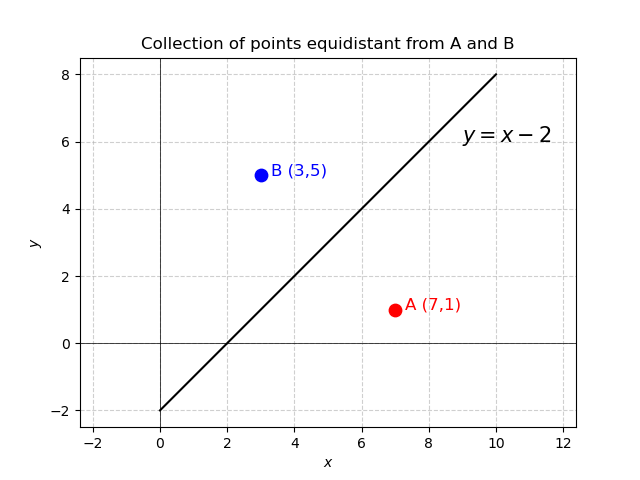
\includegraphics[width=1\columnwidth]{figs/plt.png}
\caption{Locus of $\vec{P}$ equidistant from $\vec{A}$ and $\vec{B}$}
\label{fig:plt}
\end{figure}

\end{document}
